\documentclass{article}
\usepackage[utf8]{inputenc}
\usepackage{mathptmx}
\usepackage{microtype}

\usepackage{graphicx}
\graphicspath{{images/}}
\usepackage{subcaption}
\usepackage{float}

\usepackage{listings}
\lstdefinestyle{withframe}{frame=single}
\lstset{style=withframe}

\title{CS5234 Project Report}

\author{
  Chan Wai Hap (Axxxxxx) \\
  \texttt{ xxxxx@u.nus.edu}
  \and
  Lu Wei (A0040955E) \\
  \texttt{ wei.lu@u.nus.edu}
}

\begin{document}

\maketitle

\tableofcontents

\pagebreak

\section{Overview}
The density of a graph is defined as the number of edges divided by the number of nodes.

\begin{equation}
  \rho(G) = \frac{m}{n}
\end{equation}

Where $m$ is the number of edges and $n$ is the number of nodes of graph $G$. This is a convention we are going to use consistently for the rest of this report.

A dense subgraph is induced by a set of nodes in the original graph with many edges connecting them. The problem of finding the densest subgraph for undirected graphs is first formalized by A. V. Goldberg in 1984 (REFERENCE). He proposed a polynomial time exact algorithm for both unweighted and weighted graphs. It has been an active area research since. This class of problems are interesting not just from a theoretical perspective, they also have a lot of practical applications, such as community detection in social networks, web link spam detection for search engines, and correlation mining for gene, item or time series datasets. Such graph datasets are usually large with millions and even billions of nodes, which makes poly-time algorithm impractical. This prompts research in the direction of both distributed and approximation algorithms.

In our project, we limit the scope of our investigation to unweighted and undirect graphs. First, we explored both exact and approximation algorithms from existing literature for the densest subgraph problem, and formulated a distributed exact algorithm. For experimentation, we implemented Goldberg's exact algorithm, which we used to produce baselines for various datasets we experimented with. We then replicated and improved a MapReduce implementation of an approximation algorithm by Bahman et al. in Hadoop – a distributed big data processing framework built on top of the MapReduce computational model. Last but not least, we also adopted the same approximation algorithm to a distributed graph processing framework named Giraph. We will present challenges and key lessons learned and compare the Hadoop and Giraph implementations.

\section{Algorithms and Theory}
In this section, we will introduce Goldberg's exact algorithm and briefly cover several approximation algorithms. Lastly, we will present our distributed exact algorithms and two possible realizations.

\subsection{Exact Algorithm}
The key idea of Goldberg's exact algorithm is to convert the original undirected, unweighted graph into a flow network as illustrated below:

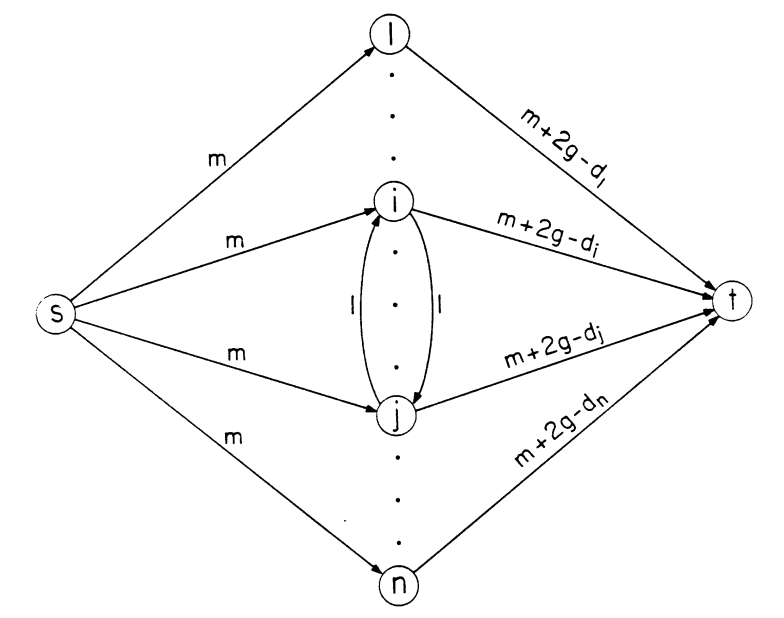
\includegraphics[width=\columnwidth]{goldberg_network.png}

Comparing to the original graph with nodes $V$ and edges $E$, the network has two nodes added: the source $s$ and the sink $t$: $V_N = V + \{s, t\}$. Every original unweight and undirected edge is converted to two directed edges each with capacity 1. The capacity from $s$ to every node in the original graph is $m$; and the capacity from every node $i$ in the original graph to $t$ is assigned $m + 2g - d_i$, where $d_i$ is the degree of node $i$ in the original graph, and $g$ is a guessed value which the algorithm is going to iteratively ``sandwich'' until it converges to the density of the densest subgraph.

The pseudocode for the algorithm is as below:

\begin{lstlisting}[mathescape=true]
  l=0, u=m, $V_1 = \emptyset$
  while $u - l > \frac{1}{n(n-1)}$ do
    $g = \frac{u+l}{2}$
    Construct network the updated g: $N = (V_N, E_N, g)$
    Find min-cut (S, T)
    if S = \{s\}
      u = g
    else
      l = g
      $V_1 = S - {s}$
  end
\end{lstlisting}

\subsection{Approximation Algorithms}
\subsection{Distributed Exact Algorithms}

\section{Implementations and experiments}
\subsection{Hadoop Implementation \& Improvement}
\subsection{Giraph Adaptation}

\section{Conclusion}

\end{document}
